\documentclass[runningheads,a4paper]{llncs}

\usepackage[utf8]{inputenc}
\usepackage[spanish,activeacute]{babel}
\setcounter{tocdepth}{3}
\usepackage{graphicx}
\usepackage{subfigure}
\usepackage{array}
\usepackage{url}

\newcommand{\keywords}[1]{\par\addvspace\baselineskip
\noindent\keywordname\enspace\ignorespaces#1}

\providecommand{\tabularnewline}{\\}


\begin{document}

%%%%%%%%%%%%%%%%%%%%%%%%%%%%%%%   TITLE   %%%%%%%%%%%%%%%%%%%%%%%%%%%%%%%

\title{Factores de influencia por género en la elección de Grados relacionados con la Tecnología}
\titlerunning{Factores de influencia por género en la elección de Ingenierías}

%%%%%%%%%%%%%%%%%%%%%%%%%%%%%%%   AUTHORS   %%%%%%%%%%%%%%%%%%%%%%%%%%%%%%%

\author{Paloma de las Cuevas, Maribel García Arenas \inst{1}}
\authorrunning{P. de las Cuevas et al.}

\institute{Dept. de Arquitectura y Tecnología de Computadores, Universidad de Granada}

\maketitle

%
%%%%%%%%%%%%%%%%%%%%%%%%%%%%%%%%%   ABSTRACT   %%%%%%%%%%%%%%%%%%%%%%%%%%%%%%%%%
%
\begin{abstract}
Ante la tendencia decreciente de la matriculación de mujeres en las ingenierías, y a la necesidad no cubierta desde Europa de incorporación de ingenieros e ingenieras al mundo laboral, se plantea un problema a resolver, que es cómo hacer las ingenierías más atractivas para los y las adolecentes.
Se debe hacer esta distinción entre chicos y chicas puesto que los factores por los que finalmente no estudian una ingeniería son distintos. Esto quiere decir que a ambos sexos les afecta una serie de factores derivados del entorno, de su percepción hacia ellos mismos y hacia los diversos aspectos de las ingenierías, pero que además el hecho de que existan una serie de estereotipos afecta a las chicas por separado.
En este artículo se presenta un análisis de los factores de influencia, y en profundidad de los factores de género, que afectan a la decisión de escoger una carrera, en este caso particularizando en las ingenierías.
Además, se ha observado e identificado la influencia de dichos factores en un contexto de centro secundaria en Granada, en el que se han realizado una serie de encuestas a alumnos de Educación Secundaria Obligatoria, Bachillerato, y Ciclos Formativos relacionados con la Tecnología y la Informática.

\keywords{...}
\end{abstract}

%%%%%%%%%%%%%%%%%%%%%%%%%%%%%%%   INTRODUCTION   %%%%%%%%%%%%%%%%%%%%%%%%%%%%%%%
%
\section{Introducción}
\label{sec:intro}

Ante la creciente necesidad de ingenieros e ingenieras en Europa \cite{gago2004europe}, los gobiernos europeos se han movilizado para intentar que crezca el interés por las ingenierías en los niveles de las enseñanzas medias \cite{Kearney2014}. Lo que es más, según la OECD\footnote{Organisation for Economic Co-operation and Development} \cite{OECD2006}, la representación femenina en carreras relacionadas con la ciencia y la tecnología permanece debajo del 40\%. En lo referente a España, la media de mujeres en las ``Enseñanzas Técnicas'' es apenas de un 31\%. El cambio al Plan Bolonia \cite{fernandez2009plan} no ha mejorado esta situación, sino que la media de mujeres matriculadas en Grados de Enseñanzas Técnicas cae y no llega al 25\% (Fuente de datos: \cite{datos::uni}.).

El propósito de este artículo es el de clarificar si los factores encontrados en la literatura son válidos para un instituto de la provincia de Granada, en el cual se ha realizado un estudio mediante encuestas a estudiantes de 3º y 4º de E.S.O.\footnote{Educación Secundaria Obligatoria}, 1º y 2º de Bachillerato, y Ciclos Formativos. Para ello, en primer lugar se identificarán en la sección \ref{sec:factores} los factores que diversos estudios encontrados en la literatura han identificado como determinantes para la elección de ingenierías. Después, en la Sección \ref{sec:EdA} se estudiará el Estado del Arte según las propuestas existentes para tratar de equilibrar las cifras en cuanto cantidad de mujeres matriculadas en Enseñanzas Técnicas. La Sección \ref{sec:metodologia} detalla el contexto en el que se han hecho las encuestas, además de las razones por las que se han escogido cada una de las preguntas, así como las fuentes. Por último, en la Sección \ref{sec:resultados} se analizan los resultados obtenidos, según los tres bloques de Secundaria, Bachillerato y Ciclos Formativos, para en la Sección \ref{sec:conclusiones} ofrecer las conclusiones sobre este estudio y unas nociones sobre el trabajo futuro.

\section{Factores de influencia identificados en la literatura}
\label{sec:factores}

A la hora de identificar los factores que tienen influencia sobre los adolescentes para escoger carreras de ingeniería, no sólo nos interesa estudiar la literatura por los factores que influyen en general, sino también en función del sexo. De un estudio realizado en la Comunidad Autónoma de Cataluña \cite{everis2012}, realizado a alumnos de 3º y 4º de E.S.O. y de Bachillerato, se pueden extraer varias conclusiones. A modo general, es decir, sin tener en cuenta el sexo del alumno que responde a las encuestas, se han encontrado con que:

\begin{itemize}
  \item Los estudiantes que van mejor en asignaturas relacionadas con la tecnología, como Matemáticas, Física, Tecnología e Informática, tienden a continuar la rama tecnológica y tienen más probabilidad de querer estudiar una ingeniería. Por contra, los que van peor suelen escoger otras ramas u otras carreras universitarias.
  \item Por lo general, menos del 33\% de los alumnos de la rama de ciencias tienen claro que quieren estudiar una ingeniería.
  \item Tanto en la E.S.O. como en Bachillerato, los alumnos escogen o no una ingeniería en función de si se ven capaces para estudiarla. Este hecho se acentúa en las chicas, quienes en general se infravaloran más y tienden a creer que más que porque sea difícil, es porque ellas no se sienten capaces.
  \item El interés por las nuevas tecnologías no es determinante en la elección de ingenierías por parte de los alumnos y alumnas. También, aunque en menos medida que la capacidad, influyen de manera directamente proporcional la percepción, positiva o negativa, que tienen sobre las salidas profesionales que tienen o el prestigio que tienen los ingenieros.
\end{itemize}

Dentro de los resultados cabe destacar que, aunque no se observen estereotipos del tipo ``friki'', sí que es notable la visión sexista que se tiene de estas carreras. Así, hasta un 60\% de los encuestados totales ve las ingenierías como ``para hombres'', mientras que solo un 42\% las considera también ``para mujeres''. De hecho, cuando se les pregunta directamente por su sexo, los resultados muy similares. En la E.S.O., dentro del 33\% total que dice que va a estudiar un Bachillerato de ciencias, hay una diferencia del 14\% entre chicas y chicos al escoger estudios relacionados con las carreras tecnológicas En el caso de Bachillerato, el 27\% de los encuestados asegura que va a continuar estudiando una ingeniería, aumentándose la diferencia entre chicas y chicos a un 31\%. El nivel socioeconómico acentúa aún más esta situación.

A la luz de estos resultados, es de interés estudiar más a fondo los factores que influencian, en particular, al colectivo femenino en la decisión de estudiar ingenierías. Para ello, se analiza el informe aportado en el proyecto ``Mind the Gap''. En este informe \cite{mtg2015} se comparan tres informes previos sobre la situación de la mujer en la tecnología y en las carreras de ingeniería en los países de Holanda, Reino Unido y España.
Hay varios puntos en común entre los tres países, entre ellos que el entorno de las chicas es uno de los factores más influyentes, sobre todo la familia. Es más, influye el hecho de la concepción de la familia, observándose entre las entrevistadas que la percepción de un trabajo de muchas horas concilia poco ``con sus tareas familiares''.

Otro factor en común entre los tres países es la poca confianza que las chicas tienen en sí mismas en cuanto a enseñanzas técnicas se refiere, que encima se ve minada por la alta presencia de hombres en carreras STEM, no ayudando a que este entorno sea cómodo para ellas. Los profesores representan otro factor importante, ya que no saben cómo actuar ante la situación que se describe a pesar de que admiten que existe.
Los resultados del informe del proyecto ``Mind the Gap'' se repiten en la mayoría de los encontrados en la literatura. Por citar algunos, en \cite{hill2010so} la AAUW\footnote{Asociación Americana de Mujeres Universitarias, o en inglés \textit{American Association of University Women}} investigó las razones de por qué hay tan pocas mujeres en las carreras o profesiones STEM, llegando a la conclusión de que las principales razones serían: la antigua creencia de que los chicos son mejores en matemáticas que las chicas, cuando este hecho se ha probado erróneo en la actualidad; el supuesto poco interés de las chicas por las STEM; y en el ámbito de empresas STEM, la conciliación familiar. 

Por último, mencionar un estudio de 2013 \cite{hazari2013factors} del que además se han incluído algunas preguntas en las encuestas realizadas y descritas en la Sección \ref{sec:metodologia}. En este estudio los autores pretenden demostrar cómo afectan realmente distintos factores, siendo el único influyente el discutir la poca representación femenina en la ciencia en clase.

\section{Estado del Arte}
\label{sec:EdA}

Según los resultados resumidos en la Sección \ref{sec:intro}, y teniendo en cuenta una de las conclusiones de uno de los estudios analizados \cite{everis2012}, que indica que se podría obtener un aumento de la vocación por enseñanzas tecnológicas con iniciativas que respondan a las necesidades de los colectivos menos representados en ellas (en este caso, las mujeres), en esta sección se presentan las iniciativas y proyectos encontrados que en la actualidad tratan de impulsar el interés de las mujeres por las ingenierías. Las propuestas encontradas son de diversa índole y, aunque todas tienen el mismo fin, se pueden clasificar en función de su manera de alcanzarlo.

\begin{itemize}
  \item \textbf{Proyectos de investigación}. Financiados por la Unión Europea o por los distintos gobiernos o universidades en distintos países, con el propósito de seguir profundizando en las razones de género por las que la figura de la mujer sigue estando muy poco representada en el mundo de la tecnología y las ingenierías. Como resultado de esas investigaciones se suelen obtener propuestas que respondan a las necesidades identificadas, pero pocas veces se llegan a implementar. Entre ellos está el proyecto ``Mind the Gap'' \cite{mtg:site}.
  \item \textbf{Agrupaciones, comunidades}. Se trata de grupos o ``clubs'' de chicas y mujeres interesadas por la tecnología, que realizan actividades de manera periódica y siempre están en activo. Pueden estar financiados por empresas, o simplemente de manera altruista. En \cite{kira2012} se citan algunas de las más importantes según el propósito.
  \item \textbf{Campamentos, campus y actividades aisladas}. Son actividades parecidas a las que se organizan en los grupos o comunidades, pero de manera puntual. Incluso aunque se realicen cada año, se trata de cursos o actividades en un tiempo limitado, tras lo cual no queda una comunidad en activo. Al igual que con las agrupaciones, pueden estar financiadas por empresas o financiarse mediante cuota de inscripción. En la Universidad de Granada se realizan actividades de este tipo cada año. En concreto, se organizan cursos anuales de dos semanas de duración para niños y niñas por una parte \cite{cinfant:site}, y sólo para chicas adolescentes por otra parte \cite{cchicas:site}.
\end{itemize}

\section{Metodología}
\label{sec:metodologia}

Al escoger la muestra sobre la que se han realizado las encuestas, dentro del Instituto de Enseñanza Secundaria Zaidín-Vergeles en Granada, se ha tenido en cuenta el contexto desde distintos puntos de vista:

\begin{itemize}
  \item \underline{Entorno socioeconómico}, que es importante conocer, puesto que como se ha visto en la Sección \ref{sec:factores}, la economía de las familias es un factor que influye de manera muy importante en la elección de ingenierías.
  \item \underline{El centro}, importante desde el punto de vista de los recursos de que dispone, ya que una buena experiencia con el material en las clases de Informática o Tecnología podría también influir en el interés de los alumnos por carreras STEM.
  \item \underline{Alumnado}, para conocer la situación global del centro antes de escoger la muestra.
  \item \underline{Profesorado}, porque también tiene relación con los recursos del centro, y porque es interesante para este trabajo analizar la proporción de profesoras y profesores en el área STEM, así como poner de manifiesto si los alumnos tienen figuras ejemplares femeninas durante su etapa formativa.
\end{itemize}

La encuesta ha sido realizada de manera presencial en las clases durante el mes de mayo de 2016, por alumnos de la asignatura de Tecnología en 3º y 4º de la E.S.O., los alumnos de clase de Tecnología en 2º de Bachillerato, los alumnos de TIC de 1º de Bachillerato, y los alumnos de Ciclos Formativos relacionados con la tecnología y la informática. La cantidad de alumnos por curso se detalla en el Cuadro \ref{tab:muestra}.

\begin{table}
  \caption{{\scriptsize Distribución de alumnos encuestados por curso.}}
  \label{tab:muestra}

  \begin{center}
    \begin{tabular}{|m{6cm}|c|c|}
    \hline
      {\small Curso} & {\small Alumnos} & {\small Enlace a la encuesta} \\ \hline
      {\small Tecnología de 3º y 4º de la E.S.O.} & {\small 63} & {\small \url{https://goo.gl/BE3Doa}} \\ \hline
      {\small Tecnología de 2º de Bachillerato y TIC de 1º de Bachillerato} & {\small 36} & {\small \url{https://goo.gl/usH9Bv}} \\ \hline
      {\small Ciclos Formativos de Enseñanzas Técnicas} & {\small 50} & {\small \url{https://goo.gl/uDuVxW}} \\ \hline
    \end{tabular}
  \end{center}
\end{table}

\section{Resultados}
\label{sec:resultados}

En primer lugar se van a obtener una serie de observaciones respecto a la distribución de respuestas en función de los distintos cursos analizados, a fin de extraer algunas conclusiones previas al estudio más profundo de las preguntas para cada curso.

La distibución de alumnos por sexo está representada en la Figura \ref{fig:alumnos_as}. La razón por la que la columna de Bachillerato suma 25, a pesar de ser 26 los alumnos totales encuestados (ver Tabla \ref{tab:muestra}) es que ha habido un alumno o alumna que no ha indicado su sexo pero sí ha respondido a las demás preguntas. La Figura muestra que en la E.S.O. es donde más paridad se encuentra, y conforme avanzan los cursos, se cumple la reducción de porcentaje de chicas. Es especialmente notable en los Ciclos Formativos, donde apenas un 8\% de los encuestados son chicas.

\begin{figure}
  \begin{center}
    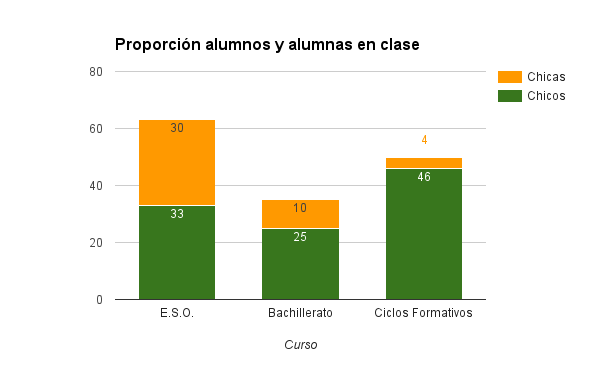
\includegraphics[width=0.7\textwidth]{Bitmap/alumnos_as.png}
    \caption{{\scriptsize Proporción de chicos y chicas en clase, en función del curso.}}
    \label{fig:alumnos_as}
  \end{center}
\end{figure}

Respecto a la elección de futuro que se plantean, según el curso, se muestra en la Figura \ref{fig:eleccion}. Para cada columna, el orden de las partes sigue el orden de las etiquetas de la leyenda, comenzando por abajo por continuación con estudios superiores, y terminando con la búsqueda de trabajo. La primera observación es que, a medida que el curso avanza en nivel, la idea de continuar estudiando se reduce y la de dejar de estudiar y buscar trabajo aumenta. En cuanto a la elección de un Bachillerato de ciencias en la E.S.O., en general hay casi el mismo porcentaje de alumnos y alumnas que lo van a escojer - un 38'10\% -, que los que escogerán otro - un 30'16\% -. Estos porcentajes bajan si nos referimos a Bachillerato, donde el porcentaje de alumnos y alumnas que dice que escogerá un grado de ingeniería es del 36'11\%, mientras que un 25\% asegura que estudiará otro tipo de grado en la universidad.

Es curioso, por otra parte, el cómo el 34\% de los encuestados en Ciclos Formativos tienen pensado hacer otro ciclo formativo más, y también relacionado con la tecnología. Esto quizá se deba a que, por lo general, los Ciclos Formativos son más accesibles que las carreras universitarias, en términos de coste y nivel académico, además de que se especializan más rápido en herramientas más actuales. Esto, muchas veces, les asegura a los estudiantes de ciclo un acceso más rápido al mercado laboral. 

\begin{figure}
  \begin{center}
    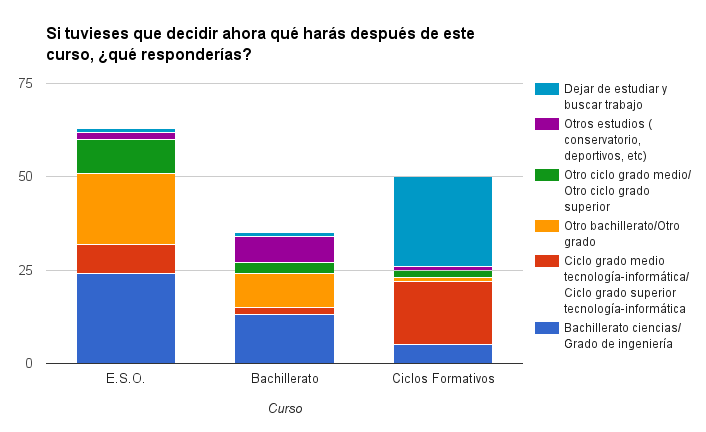
\includegraphics[width=0.9\textwidth]{Bitmap/eleccion.png}
    \caption{{\scriptsize Distribución de elección de continuación, o no continuación, de estudios según el curso. Las opciones son distintas para cada curso y se han especificado en cada leyenda. Además, en cada columna, el orden de las partes sigue el orden de las etiquetas de la leyenda, comenzando por abajo por continuación con estudios superiores, y terminando con la búsqueda de trabajo.}}
    \label{fig:eleccion}
  \end{center}
\end{figure}

El interés por las ingenieras durante la etapa de educación secundaria se muestra en \ref{fig:interes}. Mientras que a los alumnos de E.S.O. se les ha preguntado por su pensamiento actual con ``\textit{¿Cuánto dirías que te interesa la ingeniería?}'', a los demás se les preguntaba ``\textit{¿Cuánto dirías que te interesaba la ingeniería durante la E.S.O?}''. La media en todos los casos es apenas superior a 3, siendo 3'10 en la E.S.O., 3'36 en Bachillerato y 3'12 en Ciclos Formativos. Las respuestas son aproximadas, a pesar de que los alumnos de cursos superiores - sobre todo en Ciclos Formativos - podrían no recordar qué pensaban cuando estaban en la E.S.O.. Así pues, podría pensarse también que algunos siguen teniendo esa opinión y es lo que han reflejado en la respuesta.

\begin{figure}
  \begin{center}
    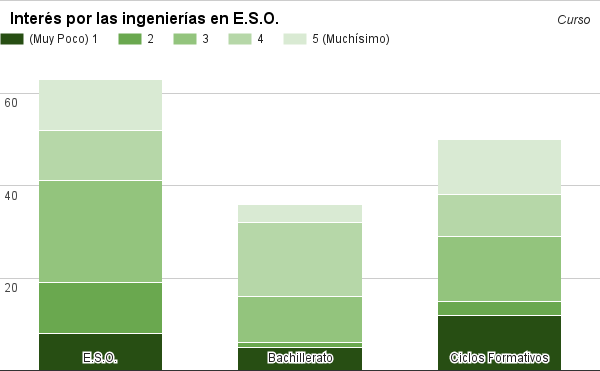
\includegraphics[width=0.65\textwidth]{Bitmap/interes.png}
    \caption{{\scriptsize Distribución del interés de los alumnos y alumnas por las ingenierías durante la etapa de la E.S.O., según el curso. A los alumnos de E.S.O. se les ha preguntado por su pensamiento actual, y a los demás por cómo pensaban cuando estaban en la E.S.O.}}
    \label{fig:interes}
  \end{center}
\end{figure}

Ahora bien, como se ve en la Figura \ref{fig:interes_tech}, el interés por las nuevas tecnologías es muy superior al registrado por las ingenierías. De hecho, en los Ciclos Formativos no ha habido nadie que haya marcado ``Muy Poco'', y solamente una persona ha calificado su interés como 2 de 5.

\begin{figure}
  \begin{center}
    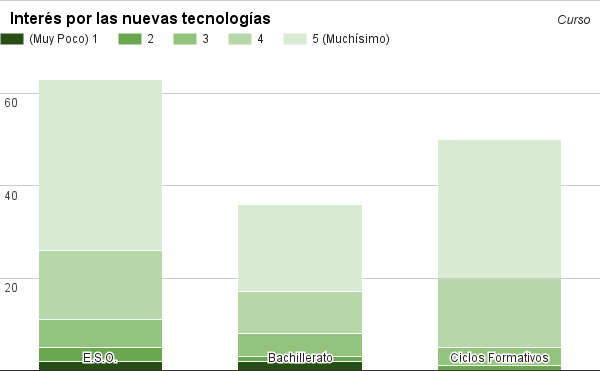
\includegraphics[width=0.65\textwidth]{Bitmap/interes_tech.png}
    \caption{{\scriptsize Distribución del interés de los alumnos y alumnas por las nuevas tecnologías, entre las que se incluían móviles, televisores inteligentes y relojes inteligentes.}}
    \label{fig:interes_tech}
  \end{center}
\end{figure}

Por otra parte, resulta curioso el hecho de que no ha habido unanimidad en ningún curso a la hora de decir si se habían organizado en el centro charlas de mujeres ingenieras, o sobre su trabajo o su poca representación en las STEM. Mientras que en la E.S.O. y en los ciclos predomina el ``No'', en Bachiller gana el ``Sí''. Se debe tener en cuenta que las encuestas han tenido lugar tras la realización de una ``Semana de la Ciencia'' que este instituto realiza todos los años. Este año \cite{ieszv:blog}, solamente una de las conferencias estaba dada por una mujer, investigadora del departamento de Física Aplicada de la UGR, si bien otra investigadora del Instituto Andaluz de Ciencias de la Tierra dio un taller. Por tanto, aún teniendo la certeza de que al menos la primera actividad por las que se preguntaba debería responderse con ``Sí'', y siendo reciente, todas las respuestas siguen el mismo patrón, ya mencionado. Se hará un análisis más profundo en cada una de las siguientes secciones.

Por último, comentar de manera general la opinión de los estudiantes sobre los Ingenieros Informáticos. Esto puede verse en la Figura \ref{fig:opiniones}. Los números indican el porcentaje de alumnos que opina que ``Sí'' es cierta esa aformación. La conclusión más clara que se obtiene es que ninguno de los encuestados cree que el trabajo de un ingeniero sea sencillo. Por otro lado, la distribución de las opiniones de los tres cursos es muy parecida, a excepción de los ciclos formativos en algunos casos. Este caso es de mucho interés, ya que en los Ciclos Formativos suele haber alumnos que ya han tenido una experiencia laboral previa.

\begin{figure}
  \begin{center}
    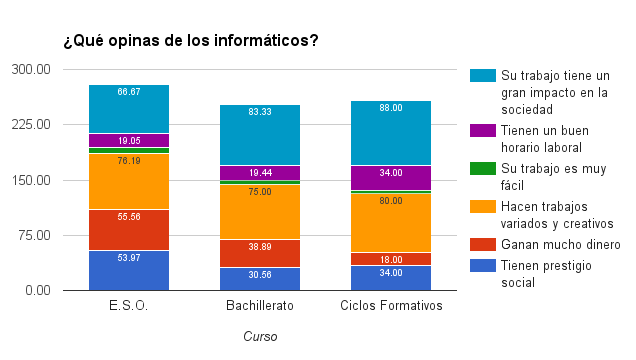
\includegraphics[width=0.9\textwidth]{Bitmap/opiniones.png}
    \caption{{\scriptsize Distribución de la opinión de los alumnos y alumnas sobre los Ingenieros Informáticos, según el curso. En cada columna, el orden de las partes sigue el orden de las etiquetas de la leyenda, comenzando por abajo por el prestigio social, y terminando con el impacto en la sociedad. Los números indican el porcentaje de alumnos que opina que ``Sí'' es cierta esa aformación.}}
    \label{fig:opiniones}
  \end{center}
\end{figure}

\section{Conclusiones}
\label{sec:conclusiones}

Como se comprueba en la Sección \ref{sec:resultados}, se han identificado todos los puntos identificados en la Sección \ref{sec:factores} en el contexto en el que se han realizado las encuestas, menos el hecho de que faltan modelos a seguir, ya que en el contexto de centro en el que se han hecho las encuestas se da el caso de que el departamento de Tecnología lo forman íntegramente profesoras. Además, se ha visto cómo a pesar de que en Bachillerato de han observado mejores notas en Tecnología e Informática por parte de las chicas, no ha habido ni una sola que haya expresado su intención de estudiar un Grado en Ingeniería.

Debido a que se ha trabajado muestra tan reducida y tan contextualizada no se pueden generalizar los resultados. A pesar de que se hayan conseguido identificar algunos de los factores que se buscaban, es claro que en el futuro se debería obtener una muestra más amplia y en diferentes contextos, como diferentes institutos provenientes de otros barrios con diferentes características. Además, se procurará escoger una fecha óptima para que las posibilidades de encontrar alumnos en las aulas sean máximas.

Se propone asimismo extender las encuestas a alumnos y alumnas de primero de Grado de Ingeniería Informática y Telecomunicaciones, para estudiar desde la perspectiva de estos alumnos las razones que les llevaron a matricularse. Incluso, como en algunos de los artículos analizados incluyen las opiniones de los profesores, se estudiará hacer un segundo bloque de encuestas a los profesores, para estudiar su perspectiva.

Por último, se continuará trabajando en iniciativas como \cite{cchicas:site} para estudiar el efecto que tienen sobre los factores analizados.

\section*{Agradecimientos} 

...


%
%Hidden for double-blind review


\bibliographystyle{splncs03}
\bibliography{eleccion_grado}


\end{document}
